%!TEX root = main.tex
\chapter{Design details / Implementation details}

Here you describe a more detailed view of the various parts of the 
architecture describing how the robot controller or game was designed.

TODO: Pakkediagram, klassediagram, (sekvens om nødvendig)
Generelt om implementasjonen, de ulike scenene/states, hovedaktører, scenemanagers/statemanagers, grafikk. Gameplay etc.  + mye mere jeg ikke kommer på i farta :D 


\begin{figure}[ht]
    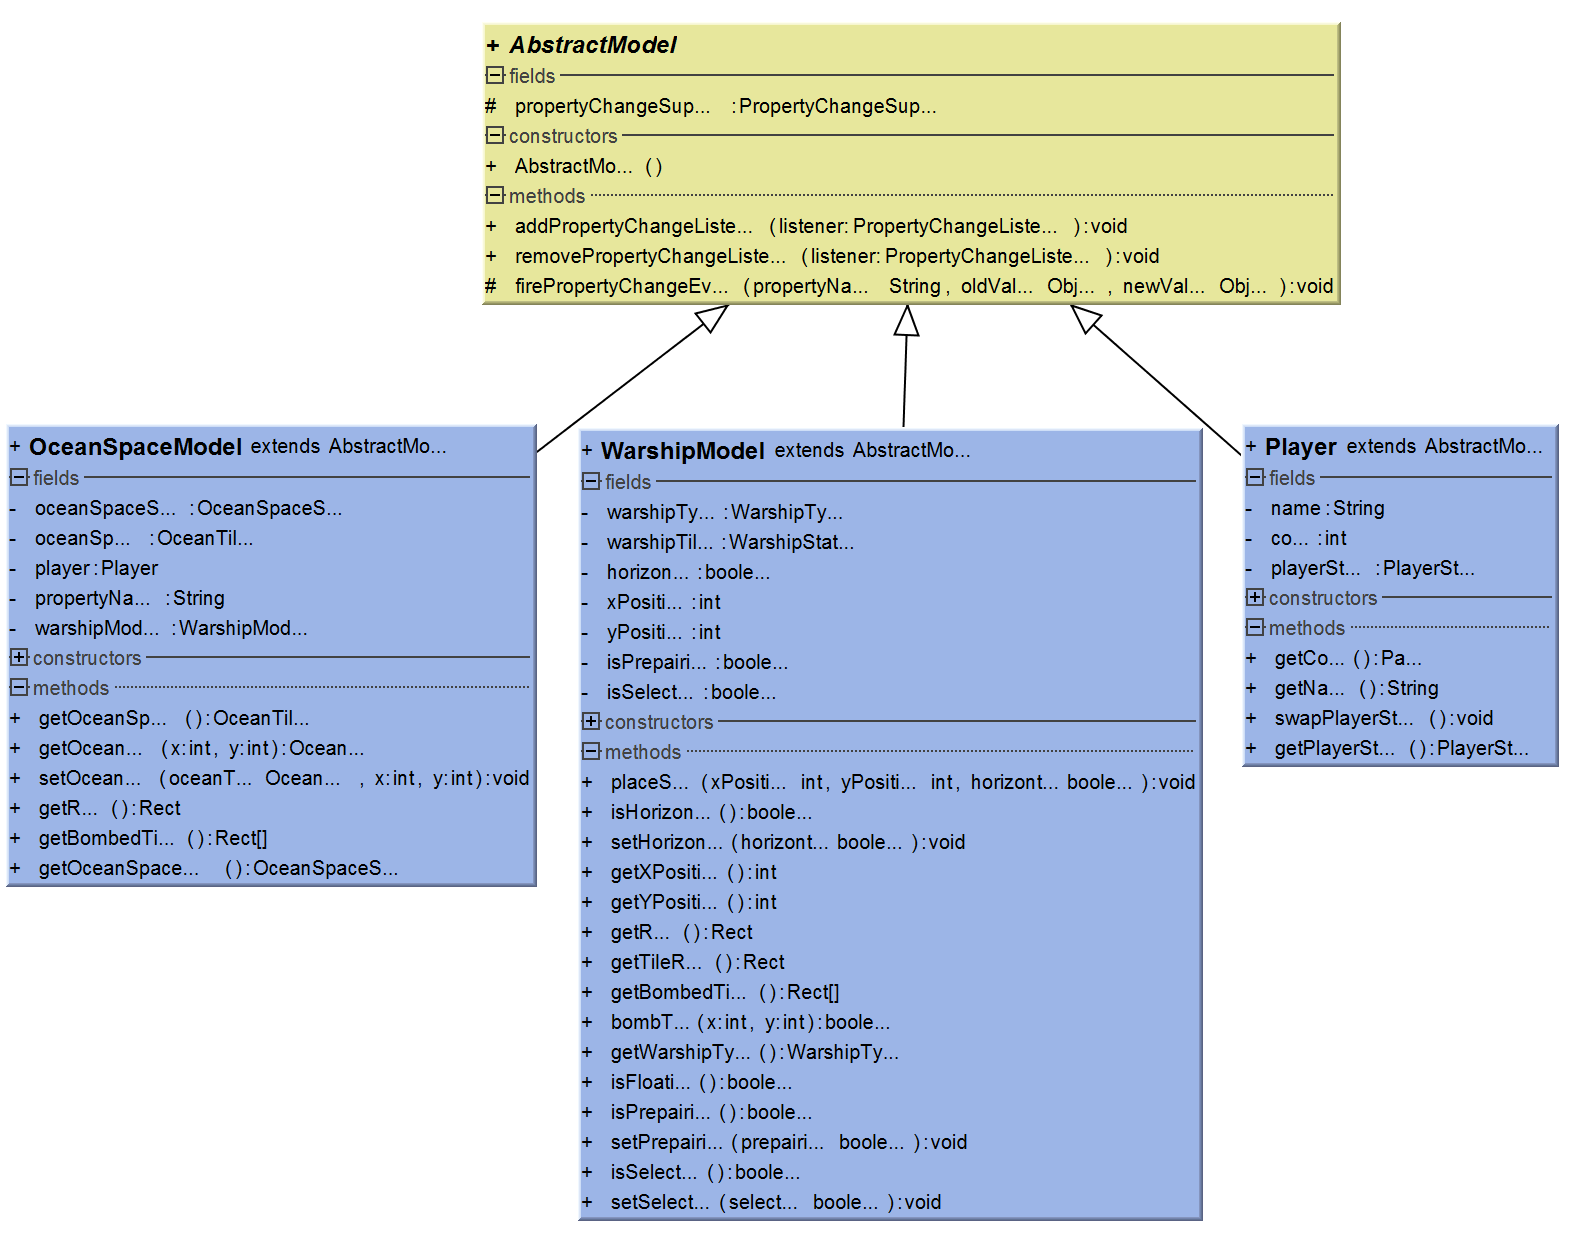
\includegraphics[width=\textwidth, angle=90]{img/Class_Model.png}
    \caption{Class diagram: Models}
    \label{fig:DevelopmentView}
\end{figure}

\begin{figure}[ht]
    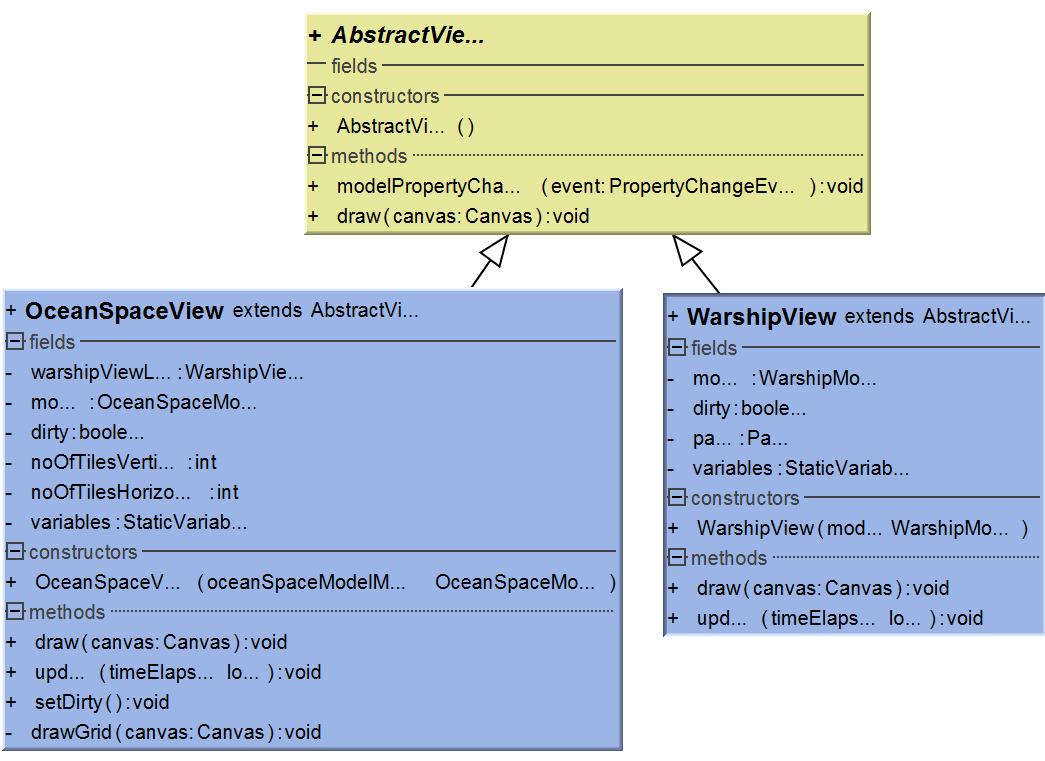
\includegraphics[width=\textwidth, angle=90]{img/Class_View.png}
    \caption{Class diagram: Views}
    \label{fig:DevelopmentView}
\end{figure}

\begin{figure}[ht]
    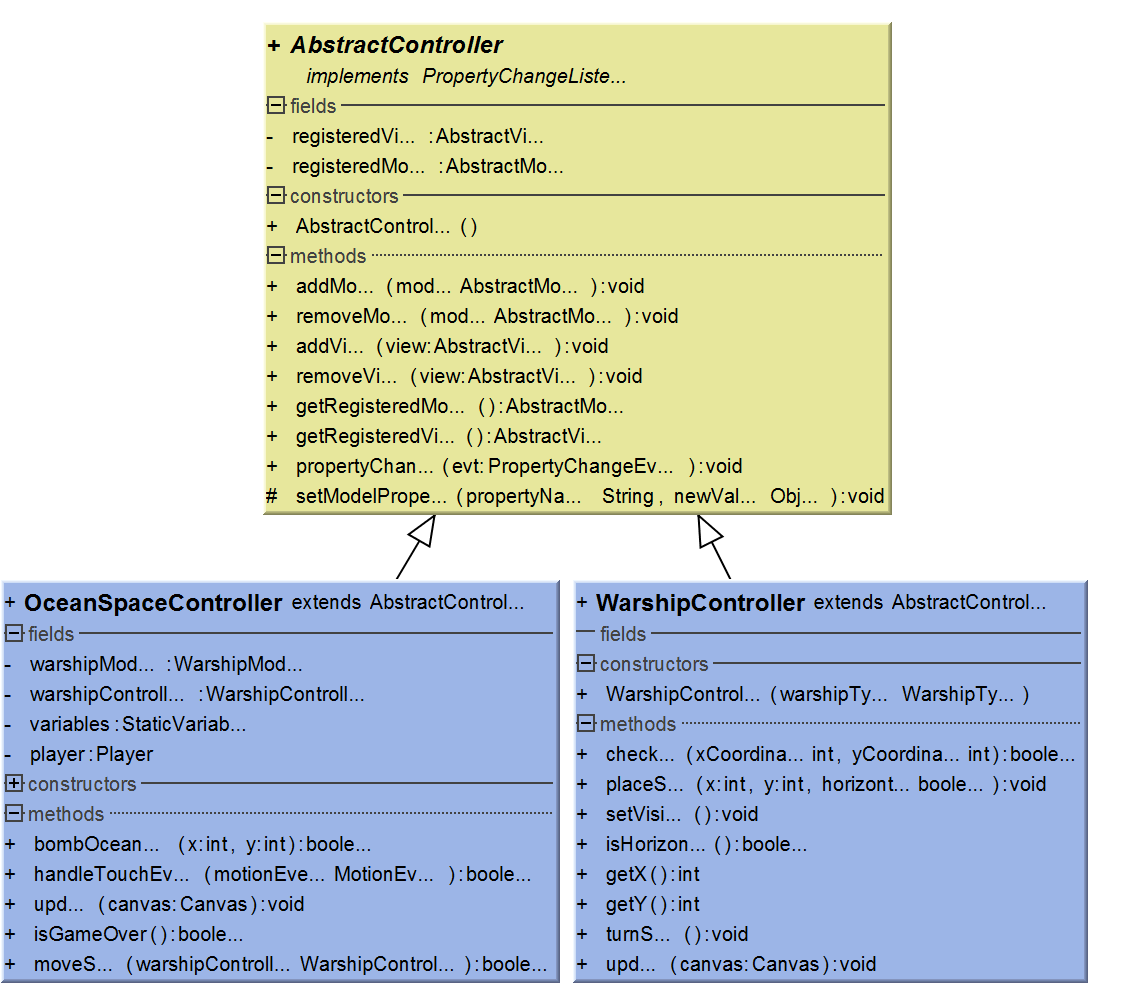
\includegraphics[width=\textwidth, angle=90]{img/Class_Controller.png}
    \caption{Class diagram: Controllers}
    \label{fig:DevelopmentView}
\end{figure}

\begin{figure}[ht]
    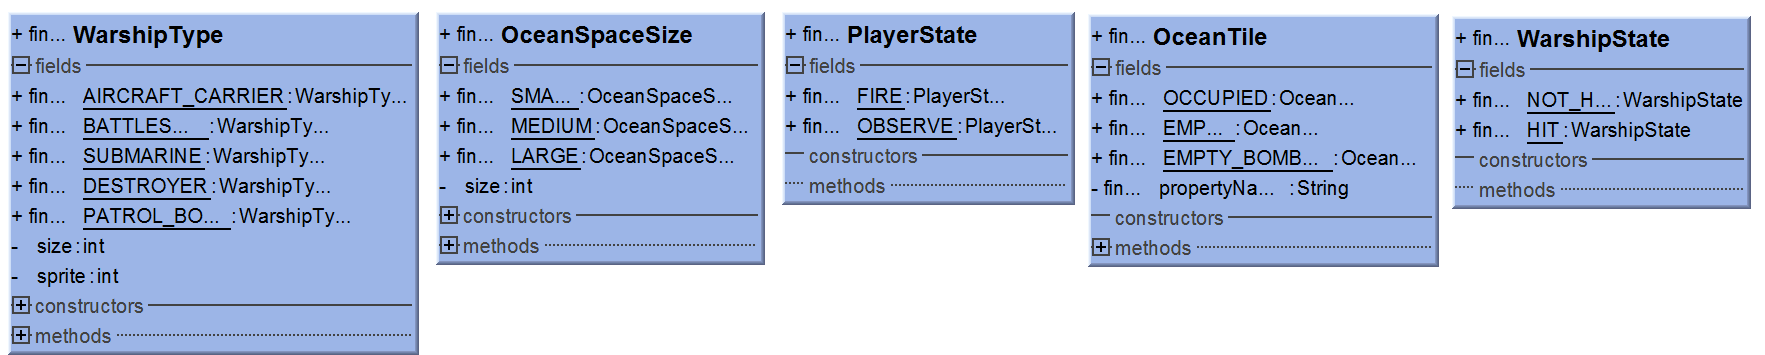
\includegraphics[width=\textwidth, angle=90]{img/Class_Enums.png}
    \caption{Class diagram: Enumerators}
    \label{fig:DevelopmentView}
\end{figure}

\begin{figure}[ht]
    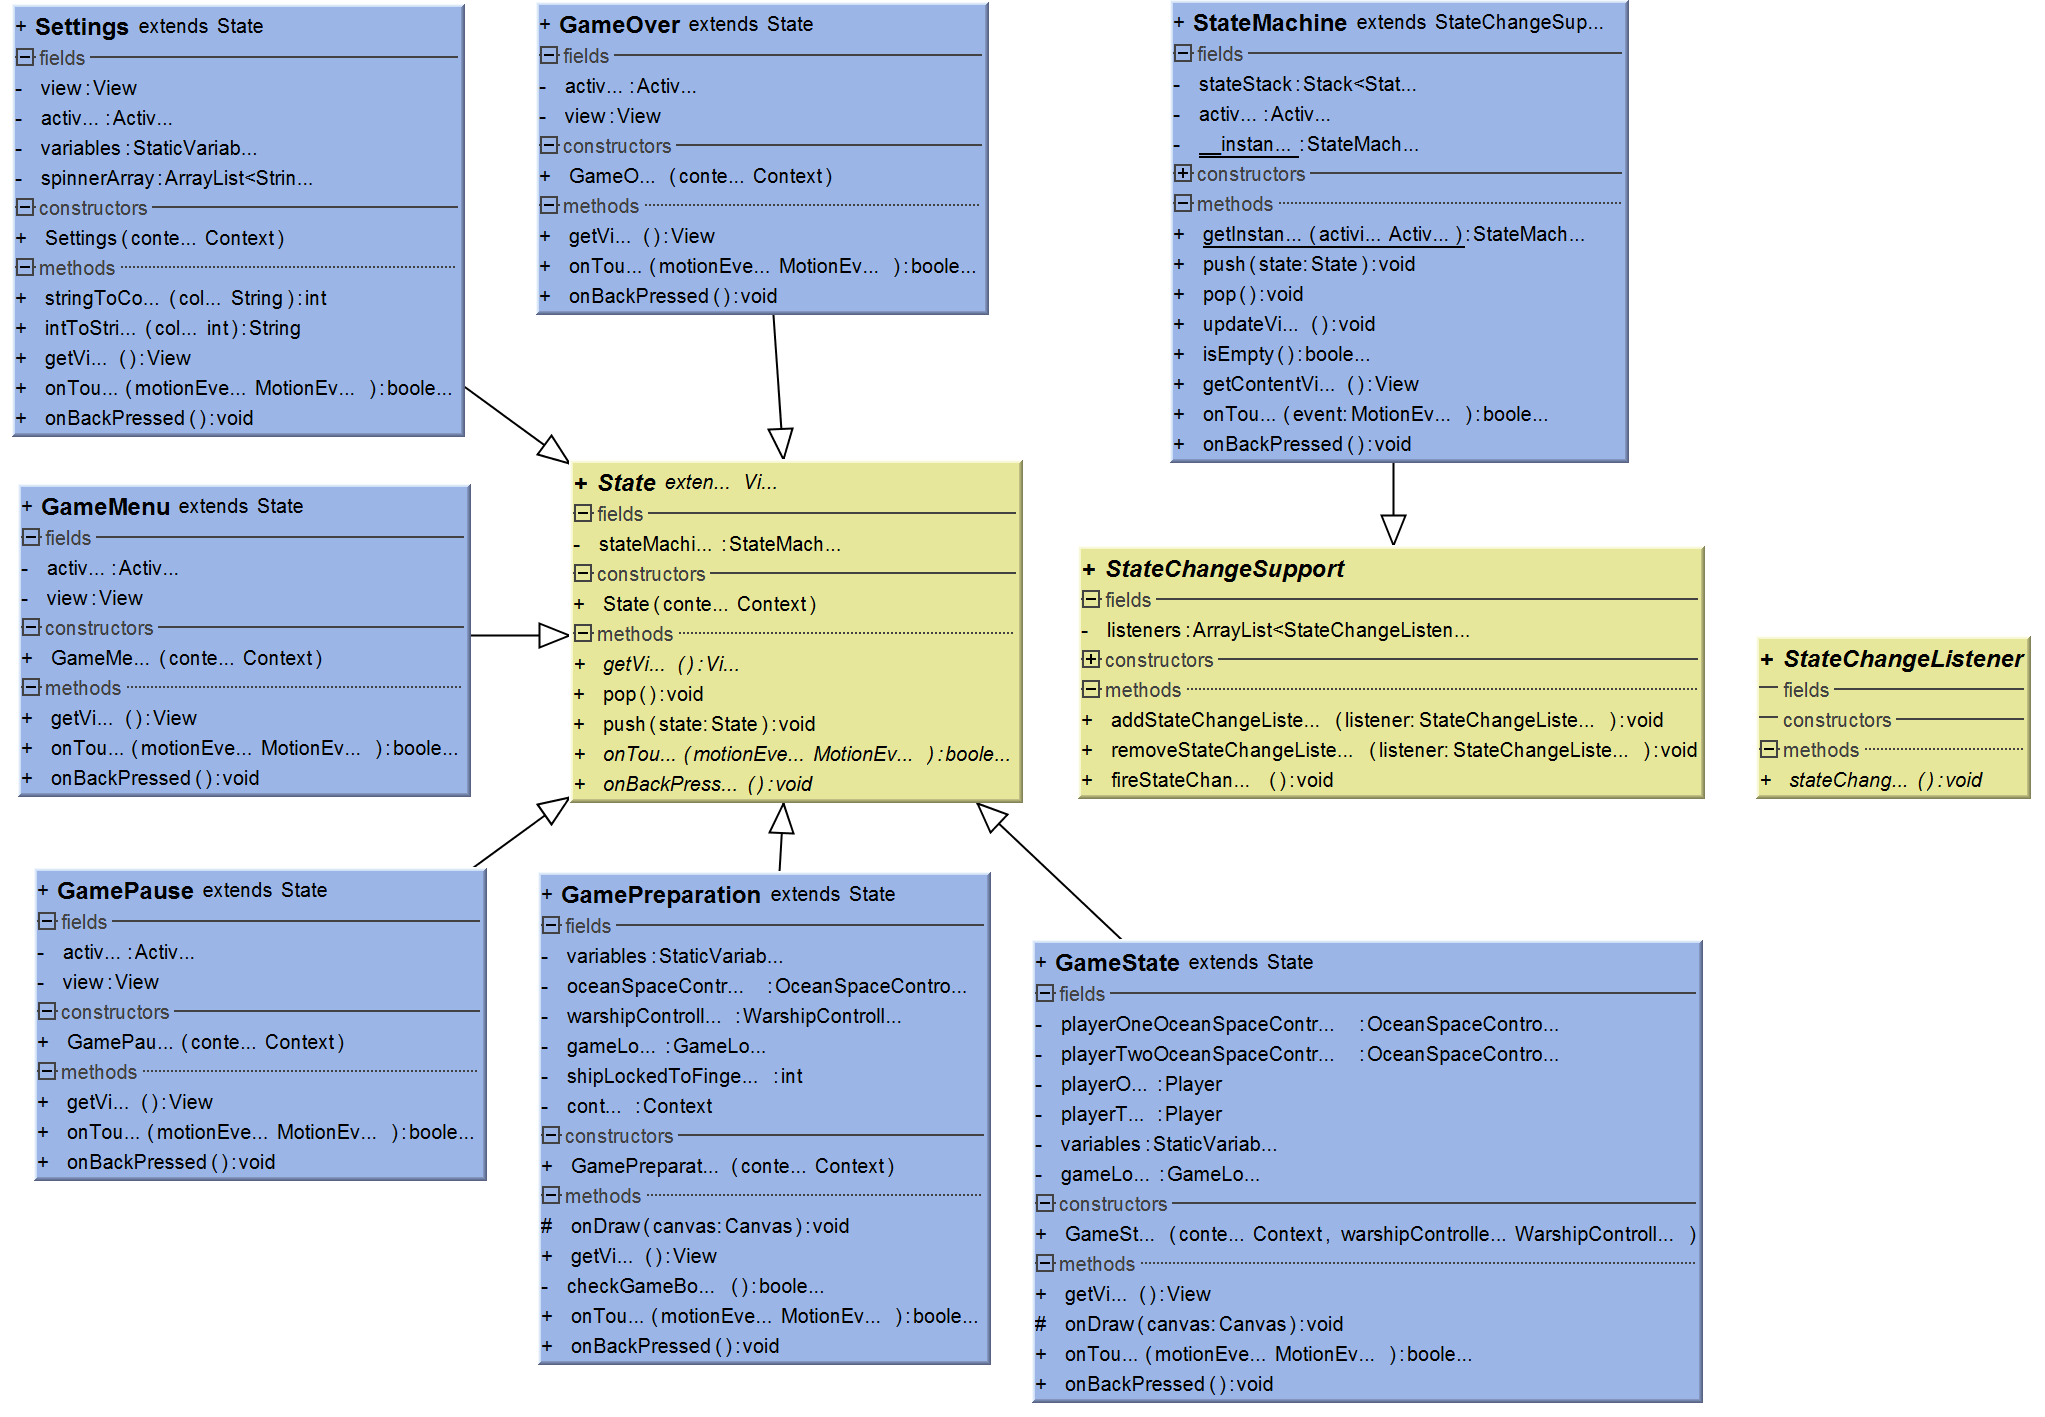
\includegraphics[width=\textwidth, angle=90]{img/Class_State.png}
    \caption{Class diagram: State}
    \label{fig:DevelopmentView}
\end{figure}

\begin{figure}[ht]
    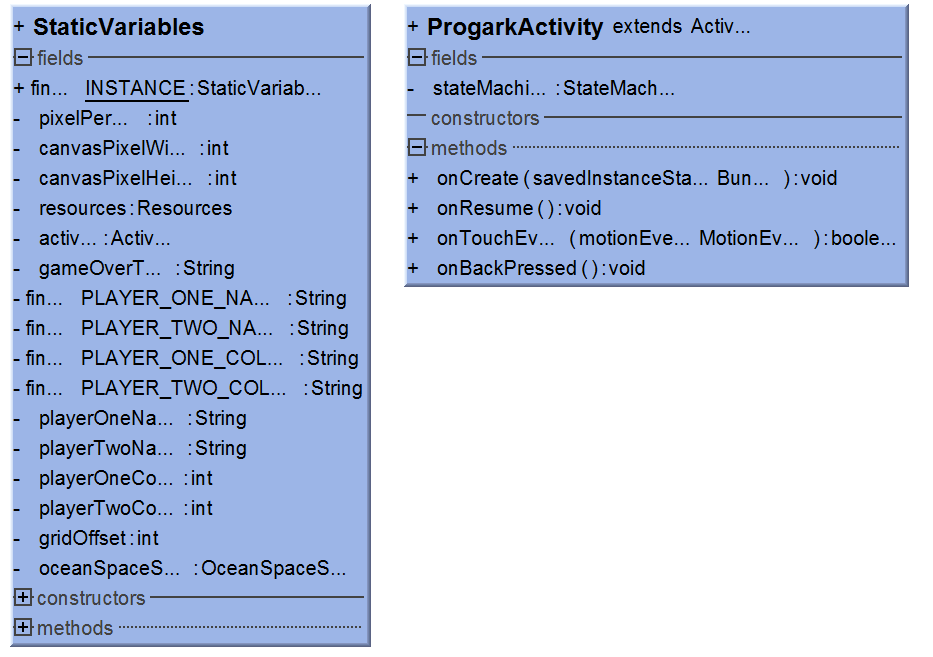
\includegraphics[width=\textwidth, angle=90]{img/Class_Misc.png}
    \caption{Class diagram: Miscellaneous}
    \label{fig:DevelopmentView}
\end{figure}